\documentclass[11pt]{article}
\usepackage[margin=1in, top=0.3in]{geometry}
\usepackage[all]{nowidow}
\usepackage[hyperfigures=true, hidelinks, pdfhighlight=/N]{hyperref}
\usepackage[separate-uncertainty=true, group-digits=false]{siunitx}
\usepackage{graphicx,amsmath,physics,tabto,float,amssymb,pgfplots,verbatim,tcolorbox}
\usepackage{listings,xcolor,subfig,caption,import,wrapfig}
\usepackage[version=4]{mhchem}
\usepackage[noabbrev]{cleveref}
\newcommand{\creflastconjunction}{, and\nobreakspace}
\numberwithin{equation}{section}
\numberwithin{figure}{section}
\numberwithin{table}{section}
\definecolor{stringcolor}{HTML}{C792EA}
\definecolor{codeblue}{HTML}{2162DB}
\definecolor{commentcolor}{HTML}{4A6E46}
\captionsetup{font=small, belowskip=0pt}
\lstdefinestyle{appendix}{
    basicstyle=\ttfamily\footnotesize,commentstyle=\color{commentcolor},keywordstyle=\color{codeblue},
    stringstyle=\color{stringcolor},showstringspaces=false,numbers=left,upquote=true,captionpos=t,
    abovecaptionskip=12pt,belowcaptionskip=12pt,language=Python,breaklines=true,frame=single}
\lstdefinestyle{inline}{
    basicstyle=\ttfamily\footnotesize,commentstyle=\color{commentcolor},keywordstyle=\color{codeblue},
    stringstyle=\color{stringcolor},showstringspaces=false,numbers=left,upquote=true,frame=tb,
    captionpos=b,language=Python}
\renewcommand{\lstlistingname}{Appendix}
\pgfplotsset{compat=1.17}

\begin{document}

\subsection{Scintillation detector theory}\label{sec:scintillator theory}
\par The two scintillation detectors used in this experiment were constructed in 2018 and 2019 respectively \cite{2018 report}\cite{2019 report}. Their design is based on the detectors used in the HiSPARC project \cite{HISPARC}, which were designed to detect cosmic rays. 
\par The detectors built at UCT were made from an EJ200 scintillation plate, a photomultiplier tube (PMT), and a light guide. They each have a cross-sectional area of \SI{0.5}{\metre^2}. The 2018 detector is labelled with 1 gold star and the 2019 with 2.

% Insert a picture of one of the detectors.

\par As charged particles of a high enough energy enter the scintillation material, they excite electrons in the material which, as they de-excite, emit photons. These photons are always the same energy, so they hold no information about the energy of the charged particle, but the number of excited electrons, and thus the number of photons emitted, is proportional to the energy of the charged particle. 
\par The photons, if left unchecked, will be emitted isotropically, so they need to be guided towards the PMT in order to be detected. To do this, the scintillation material was covered in a reflective material and a light guide was fitted to one side of the scintillation material. This fed the photons onto the cathode plate of the PMT. 
\par Once the photons hit the cathode plate, they produce an electron by the photoelectric effect. This electron gets multiplied through an avalanche effect in the PMT before being output as a voltage pulse from the anode. Details on how scintillation detectors work and how they interact with PMT's can be found in \cite{Knoll} and details on the construction of the detectors can be found in \cite{2018 report} and \cite{2019 report}.
\newline
\par The primary use of the scintillation detectors is to trigger the TRD to begin recording data. This is so that we can be sure the TRD actually has something to detect. However, the scintillation detectors only tell us when a charged particle passes through the scintillation material of that specific detector. This tells us nothing about anything passing through the TRD, so we must turn to the theory of what we are detecting in order to proceed.
\par As described in [SECTION THAT TALKS ABOUT MUON SHOWERS], when muon showers occur, they usually result in straight lines of muons that travel parallel to each other. Using this knowledge, we can set up the scintillation detectors and the TRD such that any coincident pulses from the two detectors likely come from the same muon shower event, and thus we can be fairly certain a muon was passing through the TRD at the same time. We can then collect the data from the TRD corresponding to that event and analyse it as we please.

\subsection{Using the scintillation detectors as triggers for the TRD}\label{sec:scintillators as triggers}
\par The primary use of the scintillation detectors is to trigger the TRD to begin recording data. This is so that we can be sure the TRD actually has something to detect. However, the scintillation detectors tell us when a charged particle passes through the scintillation material of that specific detector. This tells us nothing about anything passing through the TRD, so we must turn to the theory of what we are detecting in order to proceed.
\par As described in [SECTION THAT TALKS ABOUT MUON SHOWERS], when muon showers occur, they usually result in straight lines of muons that travel parallel to each other. Using this knowledge, we can set up the scintillation detectors and the TRD such that any coincident pulses from the two detectors likely come from the same muon shower event, and thus we can be fairly certain a muon was passing through the TRD at the same time. We can then collect the data from the TRD corresponding to that event and analyse it as we please.
\par The reasoning for choosing the set-up as we did is discussed further in [SECTION THAT TALKS ABOUT ANGULAR RESOLUTION], but \autoref{fig:scintillator setup} shows the set-up chosen. Ideally the two scintillators would be at the same height as the TRD chamber, but due to space constraints of the room housing the TRD chamber, they had to be placed [CAN'T REMEMBER THE DISTANCE RIGHT NOW] below the TRD chamber. Both scintillation detectors were at the same height.

\begin{figure}[h]
    \begin{center}
        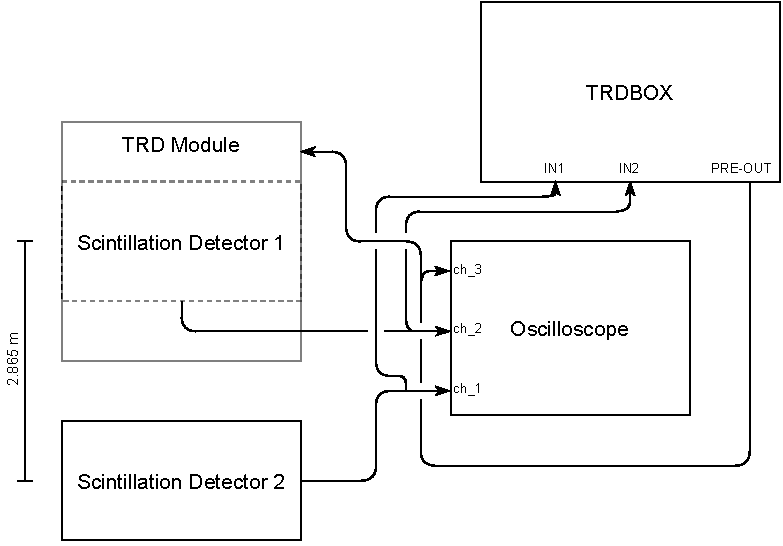
\includegraphics{Plots/setup.pdf}
        \caption{Simplified diagram of the set-up of the scintillation detectors with respect to the TRD chamber. Lengths are not to scale.}
        \label{fig:scintillator setup}
    \end{center}
\end{figure}

\par 

\begin{thebibliography}{9}
    \bibitem{2020 report} Arlow, H. Faul, S. Nathanson, N. Passmore, J. Pillay, K. Ramcharan, C. Roussos, G. Scannel, O. Thring, A. Wagener, J. Zimper, S. (2020). `Detecting and Tracking Cosmic Ray Muons using a Readout Chamber of the ALICE TRD'. UCT

    \bibitem{2019 report} Beetar, C. Blaauw, C. Catzel, R. Clayton, H. Davis, C. Diana, D. Geen, U. Grimbly, S. Johnson, D. Jackelman, T. McGregor, A. Moiloa, K. Oelgeschl\"ager, T. Perin, R. Rudner, B. (2019), `An Investigation Into the UCT-ALICE Transition Radiation Detector', UCT
    
    \bibitem{2018 report}  Barreiros, A. Barrella, J. Batik, T. Bohra, J. Camroodien, A. Govender, S. Lees, R. Rughubar, R. Skosana, V. Tladi, M. Wilkinson, J. Zeeman, W. (2018). `Detecting cosmic ray muons with an ALICE TRD Readout Chamber and commissioning a HiSPARC detector using electronic pulse processing'. UCT

    \bibitem{HISPARC} HiSPARC Project. Available at \url{https://www.hisparc.nl/en/} (2003)

    \bibitem{Knoll} Knoll, G. F., (2010). \textit{Radiation Detection and Measurement}. 4th ed. Wiley. New York.

    
\end{thebibliography}
\end{document}